\raggedbottom % Allow flexible page heights to reduce underfull vbox warnings

\chapter*{Background}
\label{chap:background}
\addcontentsline{toc}{chapter}{Background} 

This chapter provides the biological and computational background needed to understand the contributions of this thesis. We introduce the molecular biology of gene regulation, the sequencing technologies that made large-scale cellular measurements possible, the computational tasks that have emerged from these data, and the artificial intelligence methods we build upon.

\section{Molecular Biology of the Cell}

The cell is life's fundamental structural and functional unit. Its behavior is governed by gene expression: the process by which the information encoded in DNA is used to synthesize RNA and proteins, which in turn execute essentially all cellular functions. Understanding and modeling gene expression at scale is the central challenge this thesis addresses.

\begin{figure}[ht]
 \centering
 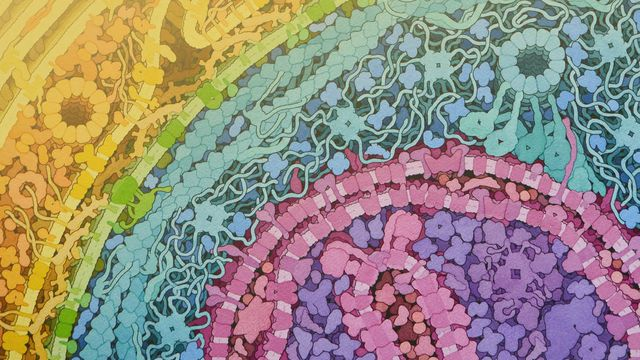
\includegraphics[width=0.9\textwidth]{./figures/aivc.jpg}
 \caption[Image of a cell]{Artist representation of a small part of a eukaryotic cell from cryo-ET images. Adopted from \citet{cellimage}}
 \label{fig:thecell}
\end{figure}

\subsection{RNA}
Among the cell's molecular components, \gls{RNA} plays a particularly central role. \gls{RNA} biology is a critical aspect of cellular function, encompassing processes such as transcription, translation, and regulation. Transcription is the process by which \gls{DNA} is copied into \gls{RNA}, which then serves as a template for protein synthesis during translation. Regulation of these processes is essential for maintaining cellular homeostasis and responding to environmental changes. This regulation can occur at multiple levels, including transcriptional control, RNA processing, and post-translational modifications \cite{Alberts2015CellsGenomes}.

Many different types of \gls{RNA} exist, each with distinct functions. Messenger \gls{RNA} (\gls{mRNA}) carries genetic information from \gls{DNA} to ribosomes for protein synthesis, while transfer \gls{RNA} (\gls{tRNA}) and ribosomal \gls{RNA} (\gls{rRNA}) allow translation of \gls{mRNA}s into proteins. Other types of \gls{RNA}, such as small interfering \gls{RNA} (\gls{siRNA}) and microRNA (\gls{miRNA}), are involved in gene regulation and silencing. Long-non-coding \gls{RNA}s (\gls{lncRNA}s) also play crucial roles in regulating gene expression and chromatin structure \cite{chenSmallLongNoncoding2024}.

\subsection{Gene Expression}
The various types of \gls{RNA} described above participate in a tightly regulated process called gene expression. Gene expression is the process by which information from a gene is used to synthesize a functional gene product, typically a protein. This process involves several key steps, including transcription, where \gls{DNA} is transcribed into \gls{mRNA}, and translation, where \gls{mRNA} is translated into a protein (see Figure ~\ref{fig:dogma}). Transcription factors (\gls{TF}s) are proteins that bind to specific \gls{DNA} sequences to regulate the transcription of genes. They play a crucial role in determining which genes are expressed in a cell at any given time, influencing cellular function and identity \cite{Alberts2015CellsGenomes}.

\begin{figure}[ht]
 \centering
 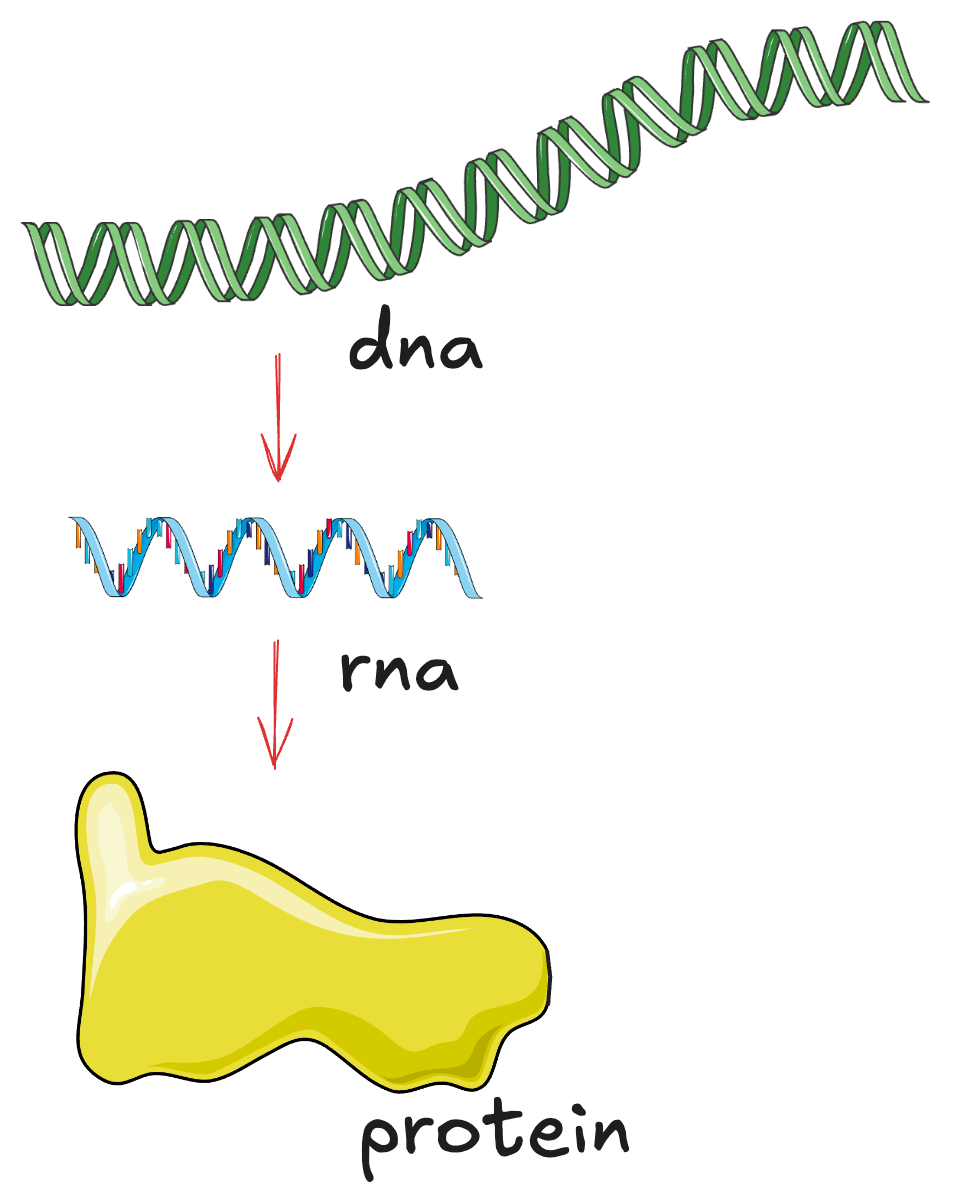
\includegraphics[width=0.4\textwidth]{./figures/dogma.png}
 \caption[The central dogma of biology]{The central dogma of biology also represents the classic view of how gene expression occurs.}
 \label{fig:dogma}
\end{figure}

Transcription factors also interact with other proteins, such as cohesin, which helps maintain chromatin and the specific 3D structure of the \gls{DNA}. Chromatin is the complex of \gls{DNA} and proteins that forms chromosomes within the nucleus of eukaryotic cells. The organization of chromatin is essential for regulating gene expression, as it determines the accessibility of \gls{DNA} to transcription machinery (see Figure ~\ref{fig:grn_1}).

Understanding the transcriptional rules governing \gls{TF} binding is central to predicting gene expression programs from genomic sequence.

\begin{figure}[ht]
 \centering
 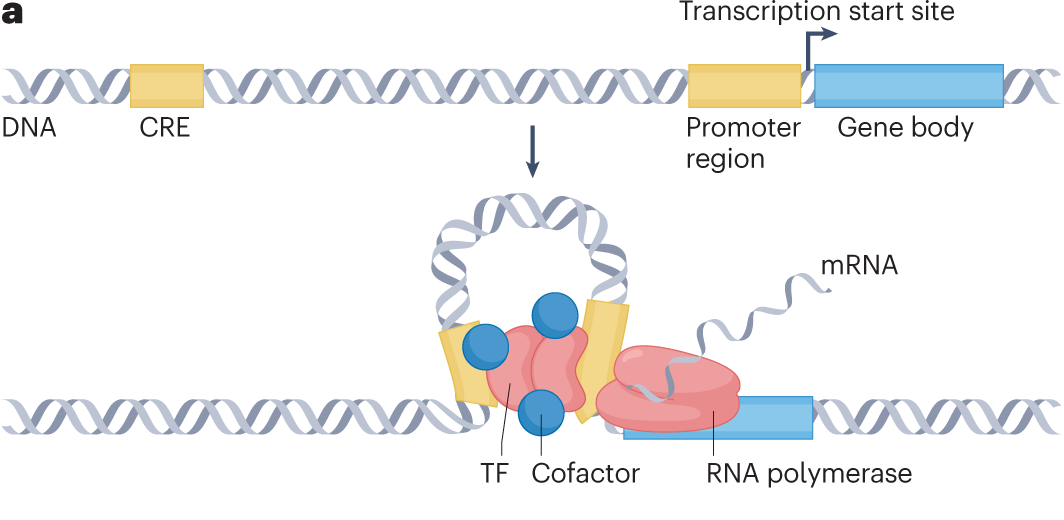
\includegraphics[width=0.9\textwidth]{./figures/grn-inference_1.png}
 \caption[Gene regulation]{Image of the classical view of gene regulation whereby transcription factors and cofactors bound to cis-regulatory elements and each other recruit the transcriptional machinery at the promoter region of the transcription start site. Adopted from \citet{badia-i-mompelGeneRegulatoryNetwork2023}.}
 \label{fig:grn_1}
\end{figure}

\subsection{Gene Regulatory Networks}
Given this complexity, biologists have relied on the concept of gene regulatory networks (\gls{GRN}s) to simplify the complex interactions within the cell \cite{badia-i-mompelGeneRegulatoryNetwork2023}. GRNs are networks of molecular interactions that govern gene expression levels in a cell. They consist of genes, transcription factors, and other regulatory elements that interact to control the timing and level of gene expression (see Figure ~\ref{fig:grn_2}). Although coarse and incomplete, these modeled interactions provide insights into how cells respond to stimuli, differentiate, and maintain homeostasis. GRNs are used operationally through pathway, regulon, and ontological relationship databases, and serve as a reference for interpreting transcriptomic data.

\begin{figure}[ht]
 \centering
 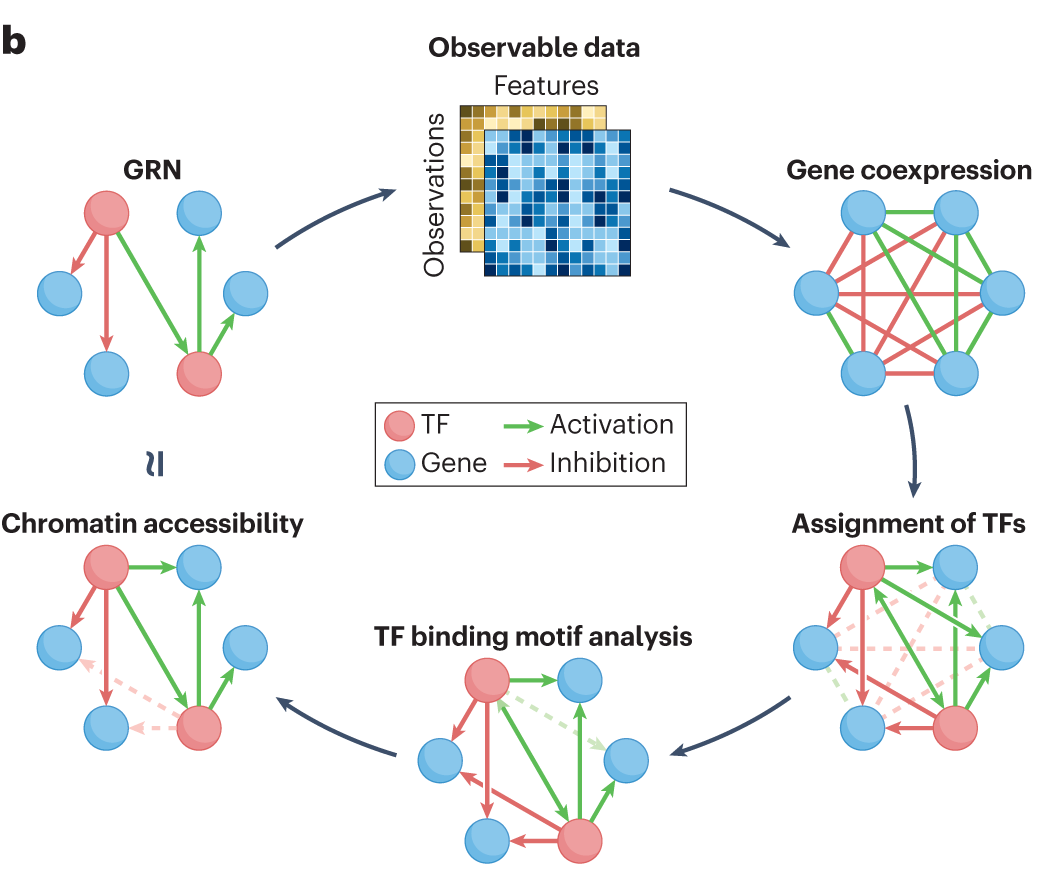
\includegraphics[width=0.9\textwidth]{./figures/grn-inference_2.png}
 \caption[Inferring gene networks]{Inferring gene networks using cellular measurements. In this loop, we see the classical approach, where multiple measurements are combined with prior knowledge and heuristics to design a network that better understands the observations and makes predictions. Adopted from \citet{badia-i-mompelGeneRegulatoryNetwork2023}.}
 \label{fig:grn_2}
\end{figure}

\section{Single-Cell Genomics}

While GRNs provide a conceptual framework for cellular regulation, measuring gene expression at scale requires advanced experimental technologies. In this section, we trace the evolution of sequencing methods from early techniques to modern single-cell approaches that generate the data our models are trained on.

\subsection{Sequencing}
The study of gene expression at scale started within the field of genomics. Genomics is the study of an organism's complete set of \gls{DNA}, including all of its genes. It involves sequencing and analyzing the entire genome to understand its structure, function, and evolution. Then, the development of high-throughput sequencing technologies revolutionized genomics, allowing researchers to sequence entire genomes quickly and cost-effectively.

Initially, \gls{DNA} sequencing was performed using Sanger sequencing (see Figure ~\ref{fig:sequencing}), the first method developed for this purpose. It involves selectively incorporating chain-terminating dideoxynucleotides during \gls{DNA} replication, enabling researchers to determine the nucleotide sequence of a \gls{DNA} molecule. This method was labor-intensive and time-consuming, but it laid the foundation for modern sequencing techniques \cite{sangerDNASequencingChainterminating1977}.

\begin{figure}[ht]
 \centering
 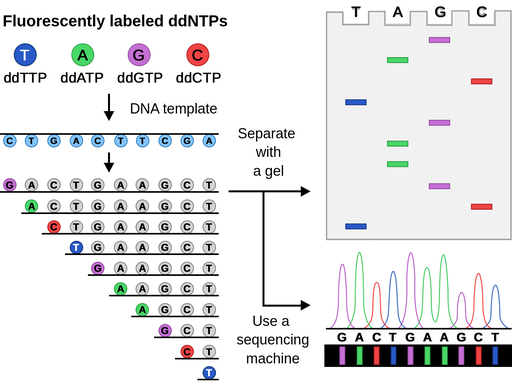
\includegraphics[width=0.9\textwidth]{./figures/sequencing_init.png}
 \caption[Main method for sequencing DNA]{Main method for sequencing DNA. Sanger sequencing uses the sequential addition of fluorescent complementary nucleotides to read the genome one nucleotide at a time. A highly parallelized version is being used in most modern sequencers. Adopted from \citet{dnamethods}.}
 \label{fig:sequencing}
\end{figure}

\subsection{Next-Generation Sequencing}
Sanger sequencing paved the way for a revolution in throughput. Nowadays, we use next-generation high-throughput sequencing (\gls{NGS}) technologies, which allow for the massively parallel sequencing of millions of \gls{DNA} fragments---also called reads---simultaneously (see Figure ~\ref{fig:illumina}). It has significantly reduced the time and cost required for genome sequencing, enabling large-scale genomic studies and personalized medicine approaches \cite{huNextgenerationSequencingTechnologies2021}.

Reads, small chunks of \gls{DNA}, often likened to tiny puzzle pieces, are multiplied and sequenced in parallel. The resulting sequences are then aligned (or mapped) to a reference genome, which serves as a template for assembling the reads into a complete genome sequence. The average number of overlapping reads that cover a specific region of the genome is called sequencing depth or coverage. Higher sequencing depth generally leads to more accurate and reliable results, as it reduces the likelihood of errors and increases the confidence in variant detection.

In the last decade, large-scale sequencing efforts such as the 1 million genomes project, the Human Genome Project, and the 1000 Genomes Project have provided valuable insights into human genetic variation and disease susceptibility \cite{1000genomesprojectconsortiumGlobalReferenceHuman2015,landerInitialSequencingAnalysis2001}. Genetic sequencing now allows us to define the genetic basis of many diseases, identify which drug might work for specific patients, and establish follow-ups for high-risk patients. It is increasingly driving clinical decisions and is becoming a standard part of patient care.

\begin{figure}[ht]
 \centering
 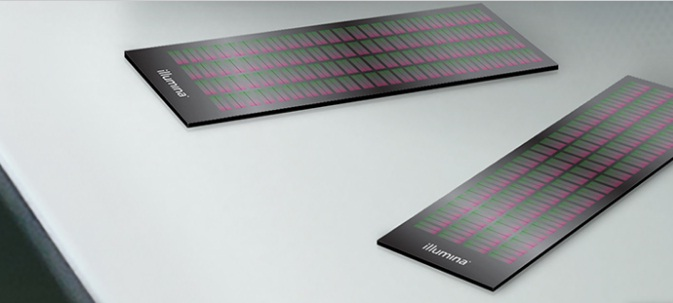
\includegraphics[width=0.6\textwidth]{./figures/illumina.jpg}
 \caption[Image of an Illumina next-generation sequencing chip]{Image of an Illumina next-generation sequencing chip. Adopted from \citet{illumina}.}
 \label{fig:illumina}
\end{figure}

\subsection{New Modalities in Sequencing}
Beyond reading the genome itself, sequencing also enabled many new applications, such as the study of gene expression. Here, we use a sequencer to read the \gls{mRNA}s present in specific tissues, a process known as \gls{RNA} sequencing (\gls{RNA-seq}) \cite{starkRNASequencingTeenage2019}. Other examples abound, such as the sequencing of \gls{DNA} states, such as methylation (\gls{BS-seq}), open chromatin (\gls{ATAC-seq}), and chromatin immunoprecipitation (\gls{ChIP-seq}), which provide a view of how the genome is being read at a point in time. From \gls{DNA} and its mutations to its state in different contexts and how these lead to changes in \gls{RNA}'s expression and state, we have begun to develop a holistic view of various cellular mechanisms \cite{buenrostroATACseqMethodAssaying2015}.

However, these methods provided only an average across cells within a tissue, not individual-cell data. In 2014, the first single-cell RNA sequencing (\gls{scRNA-seq}) methods were developed, allowing researchers to analyze gene expression at the single-cell level \cite{macoskoHighlyParallelGenomewide2015}. It was a breakthrough in genomics, enabling the study of cellular heterogeneity and the identification of rare cell populations that had previously been missed in bulk analyses.

Since then, single-cell sequencing technologies have advanced rapidly, with new methods being developed to sequence other omics modalities at the single-cell level. Studies conducted on tens of thousands of cells in the 2010s are now done on millions of cells \cite{regevHumanCellAtlas}, generating what has been called cell atlases.

In our work, we are gathering all publicly available \gls{scRNA-seq} datasets and atlases across tissues, diseases, and species to train foundation models.

\subsection{Future Directions}

\begin{figure}[ht]
 \centering
 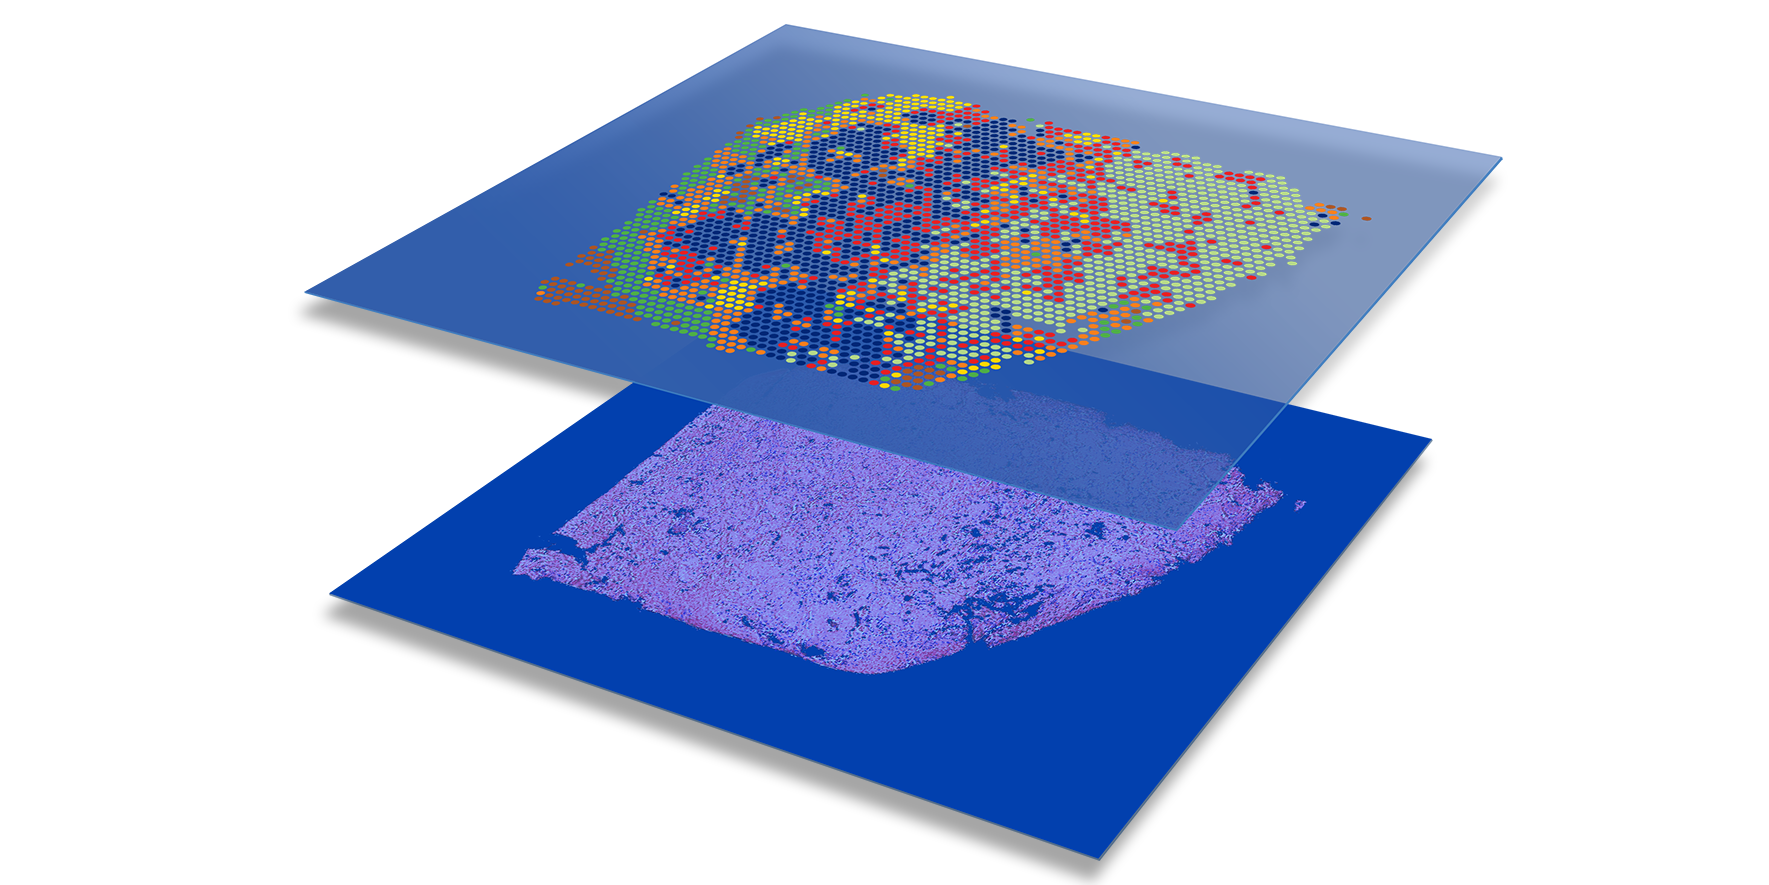
\includegraphics[width=0.6\textwidth]{./figures/spatial.png}
 \caption[Illustration of spatial transcriptomics]{Illustration of spatial transcriptomics showing how it can be used to extract additional information from a tissue slide. Adopted from \citet{tenx}}
 \label{fig:spatial}
\end{figure}

Single-cell genomics continues to expand in both scale and scope. Recently, the development of spatial transcriptomics and imaging techniques has allowed researchers to study the spatial organization of gene expression within tissues, providing a more comprehensive view of cellular function in its native context \cite{stahlVisualizationAnalysisGene2016,defardRNA2segGeneralistModel2025} (see Figure ~\ref{fig:spatial}). Protein measurements are also being developed, unlocking an additional layer of information \cite{luoAdvancesProteinSequencing2025,balezoMIPHEIViTMultiplexImmunofluorescence2025}. Current applications have primarily focused on understanding diseases and drug effects within tissues. The technique allowed the identification of hundreds of new cell types and states, and improved the study of cellular development and differentiation. It had a substantial impact on cancer, neurological diseases, and immunology \cite{josephSingleCellAnalysis2021,kongLandscapeImmuneDysregulation2023}.

Finally, the development of genetic perturbation techniques such as \gls{CRISPR}-cas9 \cite{dixitPerturbseqDissectingMolecular2016, adamsonMultiplexedSingleCellCRISPR2016}, combined with sequencing (\gls{perturb-seq}), enables us to go beyond observations and begin to understand the causal relationships between genes and their functions.

Indeed, these \gls{CRISPR} screens enable researchers to systematically knock down genes in individual cells and observe changes in gene expression, providing further insights into gene function and regulatory networks. However, these techniques are in their infancy and still limited in scale, scope, and especially, quality.

\section{Current Single-Cell Tasks}

\begin{figure}[ht]
 \centering
 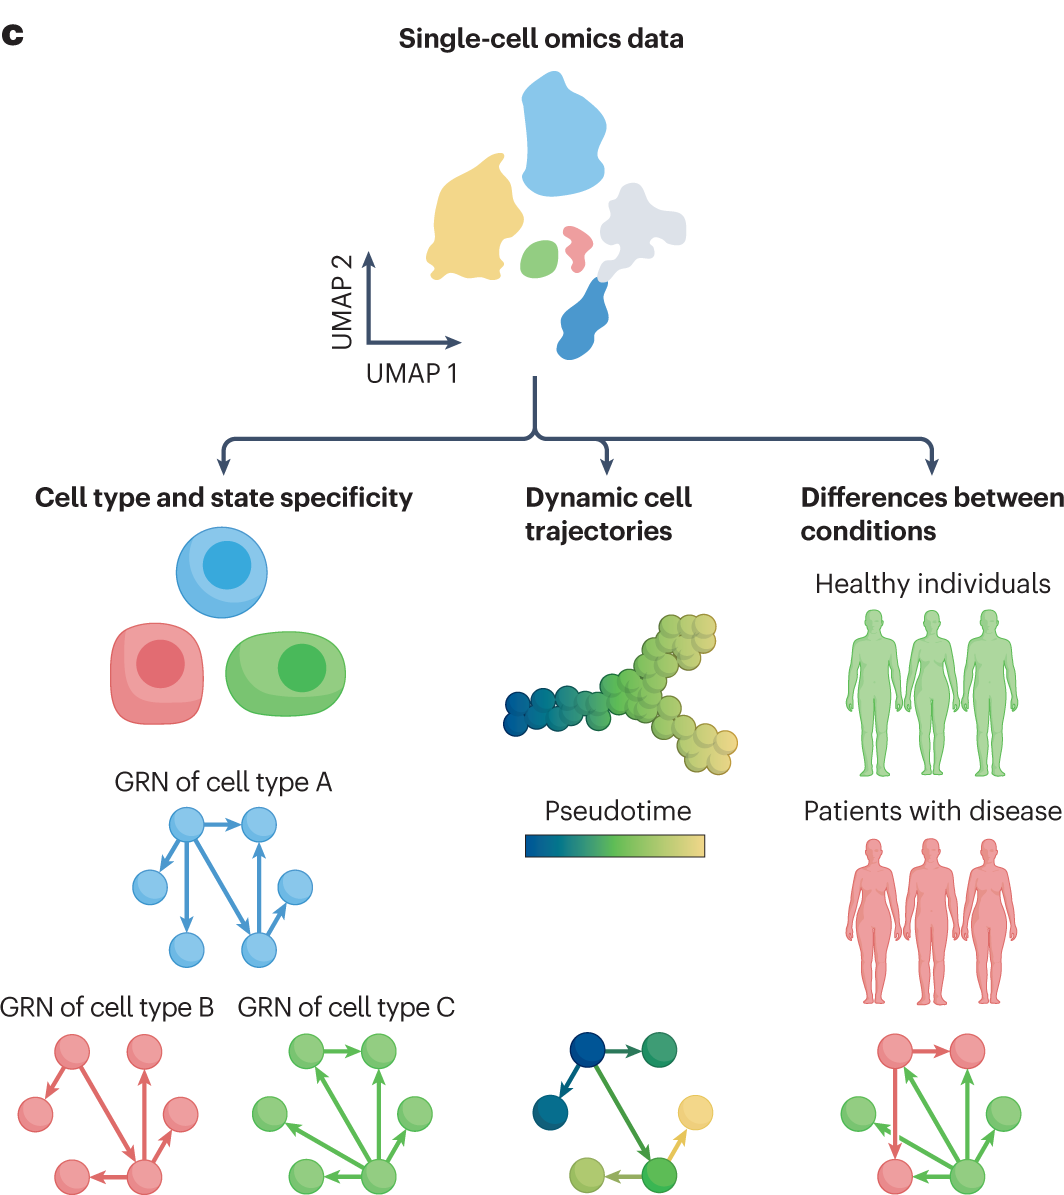
\includegraphics[width=0.6\textwidth]{./figures/grn-inference_3.png}
 \caption[Single-cell data analysis pipelines]{Single-cell data analysis pipelines and their relationship to gene networks inference. Adopted from \citet{badia-i-mompelGeneRegulatoryNetwork2023}}
 \label{fig:grn_3}
\end{figure}

The wealth of single-cell data described above has given rise to a set of standard computational tasks and analysis pipelines.
While many computational tools exist for these tasks, benchmarks that align with real use cases from the user's perspective remain scarce. Fortunately, the field has matured sufficiently to enable the creation of standardized tasks and pipelines for understanding, assessing, and analyzing data. Understanding these tasks is crucial for this thesis, as they define both our pretraining objectives and evaluation benchmarks.

In single-cell \gls{RNA-seq} data, a typical pipeline is as follows and contains several possible steps (see Figure ~\ref{fig:grn_3}). We categorize them by their role in our work: \textit{preprocessing} (applied before model training), \textit{pretraining tasks} (used to train our foundation models), \textit{zero-shot tasks} (evaluated without fine-tuning), and \textit{fine-tuning tasks} (requiring task-specific training):

\begin{enumerate}
 \item \textbf{Alignment} [\textit{preprocessing}]. It all starts with preprocessing the raw sequencing data: detecting/imputing the cell index, aligning the sequencing reads with a reference genome's gene locations, detecting low-quality cells, reads, doublet events, cell death events, and more \cite{dobinSTARUltrafastUniversal2013}. These choices will introduce biases into the output dataset. This step is performed upstream of our models.

 \item \textbf{Normalization and clustering} [\textit{preprocessing}]. The data might be normalized to correct for sequencing depth and other gene-level biases, and cell clusters would be defined based on expression profile similarity. Finally, differential expression analysis is performed, in which clusters of cells are compared to identify genes that are differentially expressed between them \cite{haghverdiBatchEffectsSinglecell2018}. Our models take normalized counts as input but learn their own expression tokenization.

 \item \textbf{Batch correction / atlas alignment} [\textit{zero-shot}]. The dataset might be aligned to a reference atlas when one exists. It is done using batch-correction methods, often built around nearest-neighbor mapping, matrix factorization, or neural networks (\gls{NN}), such as variational auto-encoders (\gls{VAE}s) \cite{scvi}. Our models perform batch correction zero-shot through learned invariant representations.

 \item \textbf{Annotation and labeling} [\textit{zero-shot / fine-tuning}]. Cluster-level and dataset-level labels might be inferred, such as cell type, tissue, disease, and age. These often come from prior knowledge, manual annotation based on differential expression features, automated tools, or alignment with other prelabeled datasets \cite{hwangSinglecellRNASequencing2018}. Our models achieve zero-shot cell-type classification via label-prediction pretraining and can be fine-tuned for specific annotation tasks.

 \item \textbf{Denoising / imputation} [\textit{pretraining task / zero-shot}]. In cases where specific clusters contain a low number of cells, denoising or zero-imputation methods can be used \cite{eraslanSinglecellRNAseqDenoising2019}, but they haven't proven consistently useful in practice because they rely on cluster-level information. We use denoising as a core pretraining objective, and our models can denoise zero-shot \cite{dijkRecoveringGeneInteractions2018}.

 \item \textbf{Multimodal integration} [\textit{not addressed}]. If users have access to datasets of the same tissue from other modalities (\gls{scATAC-seq}, \gls{BS-seq}, protein measurements, imaging, etc.), multimodal alignment methods can be applied. Such alignments help bridge the gap between genotype (e.g., \gls{DNA} mutations) and phenotype (expression, protein levels, pathology). This thesis focuses on scRNA-seq; multimodal integration remains future work.

 \item \textbf{Trajectory inference} [\textit{not addressed}]. If the dataset was measured in a non-static context, one can infer "cellular trajectories", i.e., how cells transition from one state to another based on many single-cell snapshots \cite{chenSTREAMSinglecellTrajectories2018}. We do not directly address trajectory inference in this thesis.

 \item \textbf{Spatial analysis and cell-cell interactions} [\textit{zero-shot generalization}]. If the dataset contains spatial information, one can infer cell-cell interactions based on proximity and expression profiles \cite{pallaSquidpyScalableFramework2022}. We demonstrate zero-shot generalization to spatial transcriptomics data in scPRINT-2.

 \item \textbf{Perturbation response prediction} [\textit{fine-tuning}]. If the dataset includes perturbation experiments, one can predict how cells respond to specific perturbations, such as drug treatments or genetic modifications \cite{lotfollahiScGenPredictsSinglecell2019}. We benchmark perturbation prediction as a fine-tuning task and develop counterfactual reasoning capabilities.
\end{enumerate}

These analyses and tools are available in a set of packages called scverse, which our work relies heavily on and has contributed to.

Having established the biological context and computational tasks that motivate this work, we now turn to the artificial intelligence methods that can be used to tackle them.

\section{AI and Neural Networks}

A virtual cell model has been the dream of computational and systems biologists for decades. Initially, these models were based on simplified representations of cellular processes, often focusing on specific pathways or interactions. The models examined chemical reaction parameters involving proteins, \gls{RNA}s, and \gls{DNA}. However, in addition to computational challenges, these models failed to generate realistic predictions of cellular behavior.

Nowadays, the idea has emerged that artificial intelligence techniques could help us solve some of these problems. But first, what is \gls{AI}, and what is the difference between machine learning (\gls{ML}), data science, and informatics?

\subsection{Definitions}
\textbf{Data Science} encompasses the gathering, management, and analysis of data in information systems. \textbf{Machine Learning} happens when one uses statistical methods to generate predictions from data. But while these methods can be seen in the framework of statistics, they also have an underpinning in other domains, like information systems, neuroscience (with neural networks), statistical physics, psychology, and applied mathematics (with Algebra, Topology, Analysis, and Optimization).

Artificial Intelligence (\gls{AI}) is a broad term that has had multiple meanings in society and culture. For many, it mainly refers to applications of machine learning methods to human and animal-related tasks, such as understanding images, videos, speech, and text, as well as robot manipulation. In the field, it has often been a much broader term, encompassing knowledge bases, statistical methods, and neural networks (see Figure ~\ref{fig:ffn}).

\begin{figure}[ht]
 \centering
 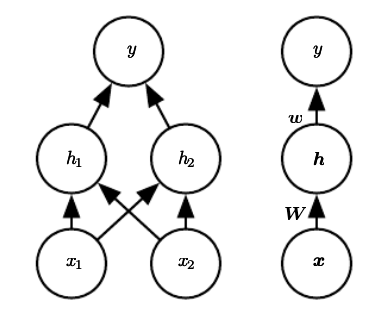
\includegraphics[width=0.4\textwidth]{./figures/ffn.png}
 \caption[Example of a feed-forward neural network architecture]{Example of a feed-forward neural network architecture, drawn in 2 different styles. Adopted from \citet{Goodfellow-et-al-2016}.}
 \label{fig:ffn}
\end{figure}

Recently, Machine Learning (\gls{ML}) has made great strides in many areas, primarily due to a significant increase in data generation, along with improvements in optimization methods and neural networks. In this Ph.D., we are piggybacking on these improvements and performing data science and machine learning on single-cell data.

We now present an overview of these methods and provide intuition for why they work.

\subsection{Learning Paradigms and Their Applications to Single-Cell Data}
Machine learning methods can be categorized into three main paradigms, each with distinct applications in our field:

\textbf{Supervised learning} involves training models on labeled data to predict outcomes. In single-cell genomics, this can include cell-type classification from expression profiles, disease-state prediction, and perturbation response modeling. These methods require curated annotations, which are often expensive and inconsistent across datasets. It is used, for example, when classifying cell type.

\textbf{Unsupervised learning} discovers structure in unlabeled data. Traditional applications include dimensionality reduction (PCA, UMAP) for visualization, clustering for cell type discovery, and matrix factorization for batch correction. It is used, for example, to learn representations of cells.

\textbf{Self-supervised generative learning} represents the paradigm underlying foundation models. It can be seen as an instance of unsupervised learning, where models are pretrained on large unlabeled datasets using proxy tasks---such as predicting masked genes or reconstructing corrupted inputs---that force them to learn meaningful representations. These representations can then be fine-tuned for downstream tasks or used zero-shot. This thesis develops foundation models in this paradigm, using denoising and expression reconstruction as pretraining objectives. Generative AI has led the second big AI revolution of this decade with tools to generate images, videos, music, voice, and text \cite{rombachHighResolutionImageSynthesis2022, shenNaturalSpeech2Latent2023, singerMakeAVideoTexttoVideoGeneration2022}.

\subsection{Representation Learning and Embeddings}
Most modern machine learning tools rely on representation learning, converting concepts and objects into high-dimensional vectors called embeddings \cite{Goodfellow-et-al-2016}. In deep Neural Networks (\gls{NN}), these embedding vectors are processed through layers of mathematical operations, often involving matrix multiplications and non-linear activation functions. The layers are designed to learn hierarchical representations of the input data, capturing increasingly complex features as data passes through the network. For single-cell data, this means learning representations in which similar cells (by type, state, or function) cluster together in embedding space, enabling downstream tasks such as classification and trajectory inference. Such tools have been heavily applied in single-cell genomics, with many methods relying on representation learning to denoise, align, and analyze data \cite{scvi}.

Recently, specific neural network architectures with powerful scaling properties, called transformers, have become ubiquitous. Researchers have extended their capabilities to scientific domains, including weather prediction \cite{lamLearningSkillfulMediumrange2023} and, as we explore in this thesis, cellular modeling. But why and how are these models so powerful? While this remains an active area of research, essential theories have been presented.

\subsection{Why Does It Work? Architectural Innovations}
Contrary to previously accepted machine learning dogma, deep learning researchers showed in the 2010s that increasing the number of parameters did not necessarily lead to overfitting. Instead, thanks to regularization methods such as dropout and weight decay, models learned more complex patterns in the data.

Several key architectural innovations enabled modern deep learning:

\textbf{Skip connections} (residual connections) prevent vanishing gradients by allowing information to flow directly across layers. This innovation led to architectures such as ResNet \cite{heDeepResidualLearning2015}, enabling the training of much deeper networks: a major component of the deep learning revolution of the 2010s. It is also widely used in transformer-based models.

\textbf{Normalization layers} (batch normalization, layer normalization) stabilize training by normalizing intermediate activations, allowing higher learning rates and faster convergence. Layer normalization is particularly important for transformers and is used in all models.

\textbf{Tokenization and attention} make the models both more parallelizable and more complex. Indeed, it allows models to work on matrix inputs, where each input value becomes a vector of numbers (also called an embedding or token). For text, this involves subword units; for single-cell data, we can let our imagination run free; it could be genes, cells, molecules, indeed, we will be using both in our models.
We then use classical neural networks for per-token processing and the attention mechanism to enable tokens to interact with one another.
Taken together, these make the model even more parallelizable in both depth and width.

\textbf{\gls{GPU}s} or Graphical Processing Units, which are the final enablers allowing us to reach unprecedented scales through large, very efficient parallel matrix operations.

These innovations are particularly relevant for genomics: attention mechanisms can capture gene-gene interactions, parallelization enables processing thousands of genes, and proper tokenization of expression values is crucial for learning meaningful representations. Indeed, they have already greatly impacted biology across multiple fronts, a famous example being the recent Nobel Prize-winning AlphaFold2 model, built on modified attention architectures \cite{jumperHighlyAccurateProtein2021}.

The final piece of the puzzle is in how we train such models.

\subsection{Optimization and Loss Landscapes}
Interestingly, whether small or large, neural network or otherwise, almost all \gls{ML} methods are trained using variants of gradient descent optimization methods. These methods aim to minimize a loss function, which quantifies the difference between the model's predictions and the actual data. By iteratively adjusting the model's parameters in the direction that reduces the loss, these optimization algorithms help the model learn from the data.

But this is through \emph{stochastic} gradient descent (\gls{SGD}) methods like Adam that we successfully train \gls{NN}s \cite{kingmaAdamMethodStochastic2017,loshchilovDecoupledWeightDecay2019}. Indeed, using only a small subset of the data at each training step is not only much faster to minimize the loss function, but it also helps escape local minima and saddle points \cite{liVisualizingLossLandscape2018}.

To understand this, we need to understand the loss landscape. Imagine a 3D landscape where the height represents the loss value, and the two other "surface" dimensions are the model's parameters (see Figure ~\ref{fig:loss_surface}). The goal of the model is to find the lowest point in this landscape, which corresponds to the best set of parameters to fit the data. However, this landscape is very complex, with many local minima and saddles, which would prevent the model from reaching a nice minimum; it wanders blindly and can only sense its immediate surroundings.

\begin{figure}[ht]
 \centering
 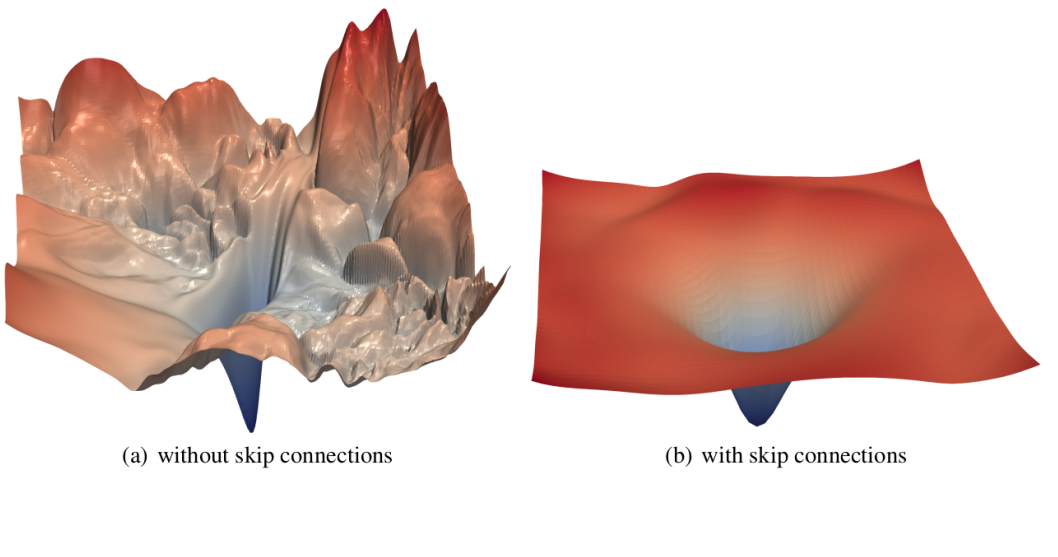
\includegraphics[width=0.9\textwidth]{./figures/loss-surface.png}
 \caption[Visualization of a loss landscape]{Visualization of a loss landscape with and without skip connections. The figure shows the loss values on the z-axis and color-coded by parameters on the x- and y-axes. Adopted from \citet{liVisualizingLossLandscape2018}}
 \label{fig:loss_surface}
\end{figure}

In deep neural networks, there are not just two but billions of dimensions, however. In this context, the loss landscape doesn't contain that many local minima; there is always a possible direction to decrease the loss. Furthermore, \gls{SGD}, by being stochastic, alters the loss landscape each time, allowing the model to easily find an escape direction from a local minimum or a saddle point (a locally flat surface).

Behind this unexpected behavior is the unsettling theory of emergence. Or how small objects can combine and interact in ways that would be unexpected and difficult to predict based on their individual properties. This theory tries to explain phenomena in dunes, snowflakes, ant colonies, and life itself, which might explain how large neural networks achieve such complex behaviors \cite{weiEmergentAbilitiesLarge2022}.

\subsection{Transformer Architectures: Encoder vs. Decoder}
For text, images, videos, and audio, large language models (\gls{LLM}s) are now ubiquitous. In scientific domains, we call similar models trained on all available data in a given modality foundation models. These models represent a paradigm shift from small, task-specific neural architectures to larger, transformer-based architectures (see Figure ~\ref{fig:transformer}), trained across entire data domains, to generalize to unseen datasets and novel tasks \cite{bommasaniOpportunitiesRisksFoundation2022}.

Two main transformer architectures exist, with different implications for genomics:

\textbf{Encoder-only models} (e.g., BERT \cite{devlinBERTPretrainingDeep2019}) use \textbf{bidirectional} attention, where each token can attend to all other tokens. This is well-suited for understanding and classification tasks. For single-cell data, bidirectional attention allows each gene to see all other genes, naturally modeling gene-gene interactions.

\textbf{Decoder-only models} (e.g., GPT \cite{brownLanguageModelsAre2020}) use \textbf{causal/unidirectional} attention, where each token can only attend to previous tokens. They are trained with \textbf{autoregressive} prediction: predicting the next token given previous ones.

In single-cell genomics, the choice is consequential: genes lack a natural ordering (unlike words in sentences), making bidirectional architectures more appropriate. Our models use encoder-style bidirectional attention, treating genes as an unordered set where each gene can attend to all others. This design choice enables learning symmetric gene-gene relationships suitable for GRN inference.

\textbf{Structured and sparse attention.} Standard attention allows every token to attend to every other token, with complexity $O(n^2)$. However, biological systems have inherent structure: genes interact through regulatory networks, proteins form complexes, and cells communicate through defined pathways, motivating variants of the attention mechanism that incorporate prior knowledge or learn sparse patterns. \textbf{Graph attention networks} \cite{velickovicGraphAttentionNetworks2018} restrict or bias attention to predefined edges in a graph, allowing tokens to attend only to their neighbors. It is particularly relevant for genomics, where protein-protein interaction networks or known regulatory relationships can guide attention.

Similar ideas were used in the development of AlphaFold2 and AlphaFold3 \cite{abramsonAccurateStructurePrediction2024a,
jumperHighlyAccurateProtein2021}. In text processing, similar examples abound of \textbf{Sparse attention} mechanisms like Longformer \cite{beltagyLongformerLongDocumentTransformer2020} and BigBird \cite{zaheerBigBirdTransformers2021}, which combine local windowed attention with global tokens, achieving linear complexity while maintaining expressiveness.

Finally, while some of these methods already decrease the computational complexity of attention, \textbf{efficient attention} methods such as hyper attention, Performer, and others \cite{choromanskiRethinkingAttentionPerformers2022, hanHyperAttentionLongcontextAttention2023, goncalvesAdaSplashAdaptiveSparse2025} approximate the attention mechanism using low-rank approximations, dropping blocks, or using kernel methods.

For single-cell models processing thousands of genes, such efficiency gains are essential. In our work, we explore how attention patterns learned during pretraining can bias them, and how we can reduce their computational complexity.

\begin{figure}[ht]
 \centering
 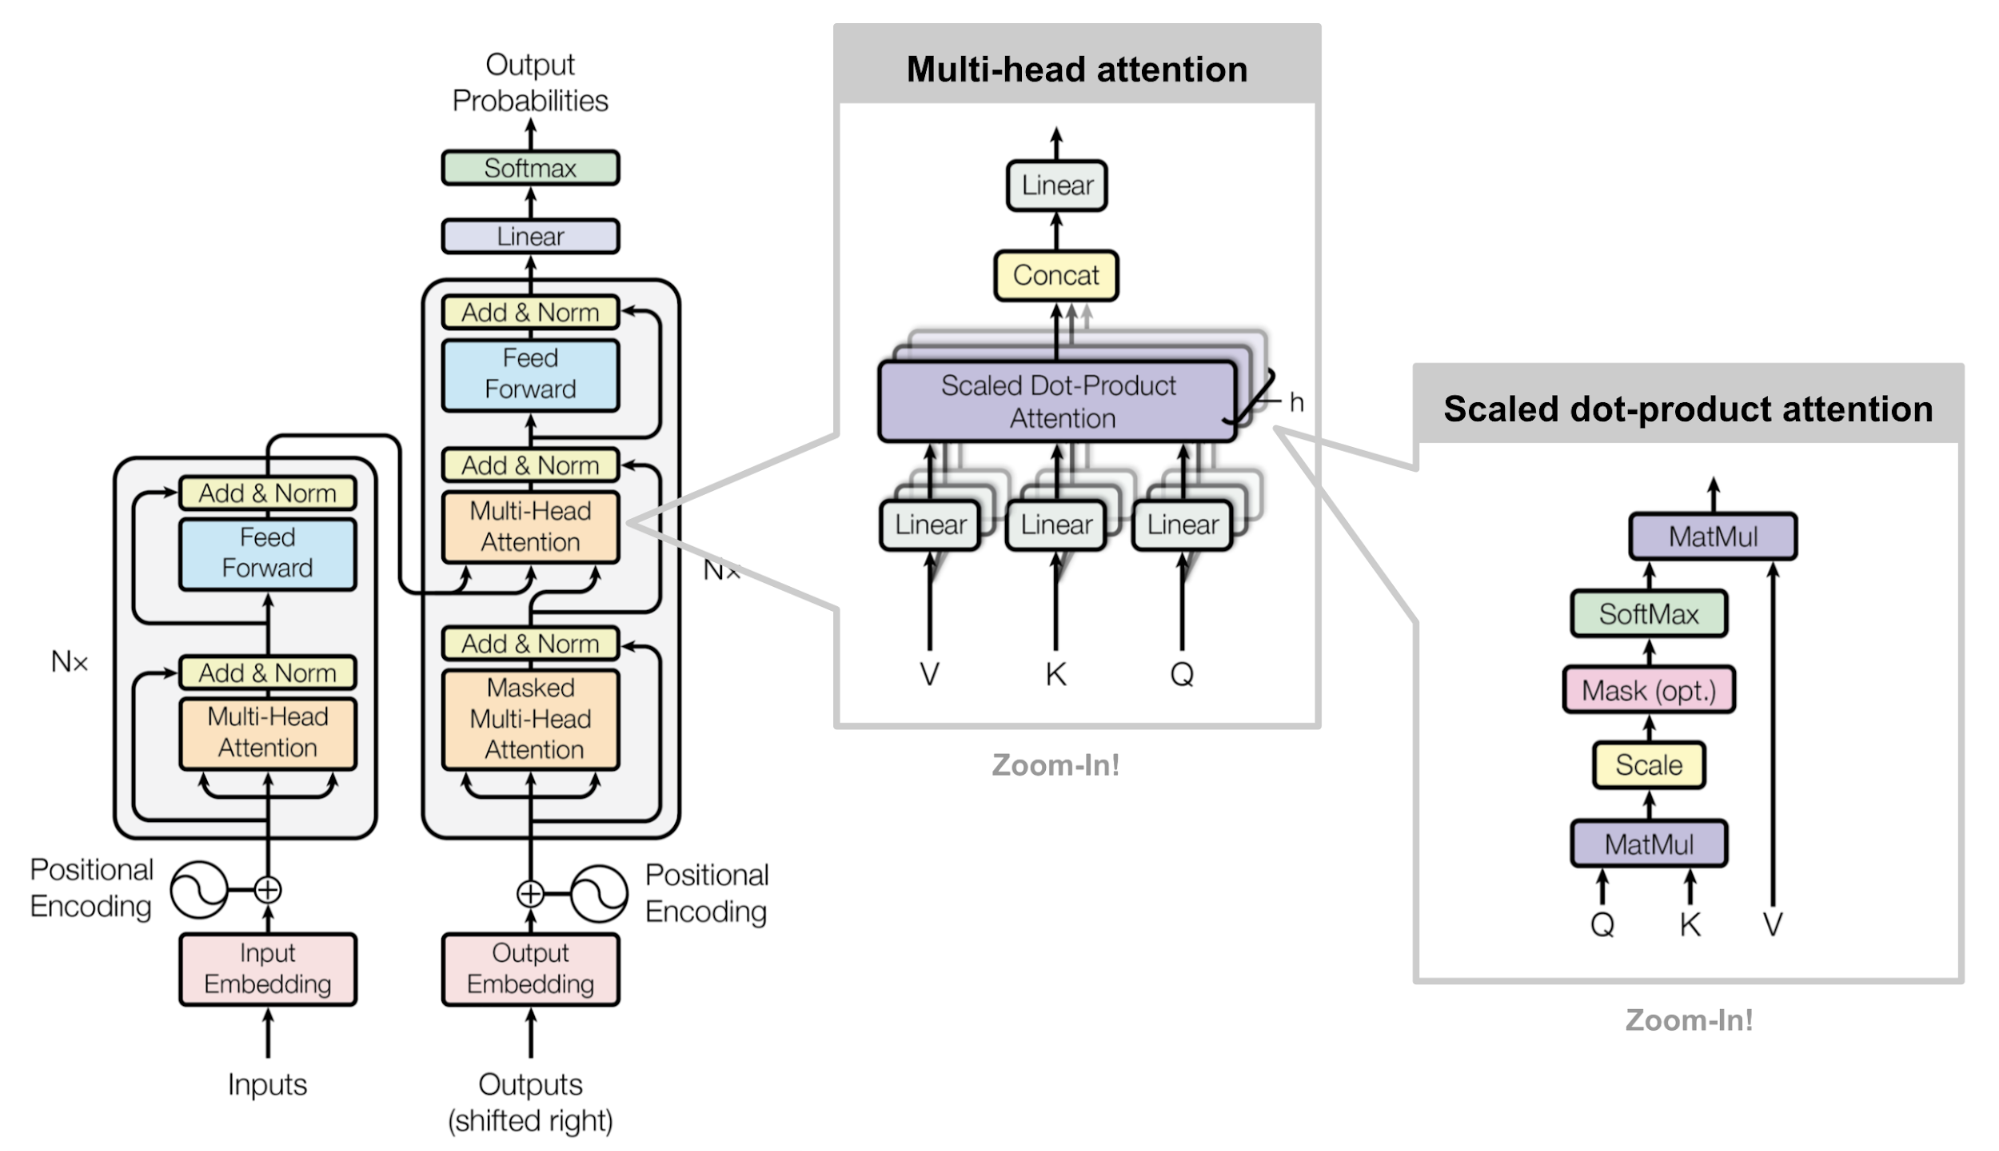
\includegraphics[width=0.9\textwidth]{./figures/transformer.png}
 \caption[Transformer architecture overview]{Transformer architecture overview. From Attention is all you need. The leftmost block is an encoder transformer, the longer block to its right is a decoder transformer. Nowadays, most methods are either one or the other, but many combinations, such as the one presented here, can be created. Adopted from \citet{vaswaniAttentionAllYou2023}.}
 \label{fig:transformer}
\end{figure}

\subsection{The Pretraining-Fine-tuning-Zero-shot Pipeline}
The foundation model paradigm involves three phases that we leverage extensively in this thesis:

\textbf{Pretraining} uses self-supervised tasks on large unlabeled datasets. For language, this is next-token prediction; for single-cell data, we use expression denoising (reconstructing original counts from corrupted inputs), bottleneck learning (compressing and reconstructing cell representations), and hierarchical label prediction. Pretraining teaches the model general patterns; for our models, this includes gene co-expression patterns, cell-type signatures, and regulatory relationships.

\textbf{Fine-tuning} adapts pretrained models to specific tasks using smaller labeled datasets. The pretrained weights provide a strong initialization, enabling faster convergence and better performance than training from scratch. We fine-tune for tasks like perturbation prediction, where limited experimental data is available.

\textbf{Zero-shot inference} applies pretrained models directly to new tasks without any task-specific training, thus testing whether pretraining has learned genuinely transferable representations.

In this thesis, we will examine pretrained foundation models in both their zero-shot and fine-tuned abilities, but we are most interested in the representations they learn during pretraining.

This pipeline is particularly valuable for biology, where labeled data is expensive and inconsistent. By pretraining on millions of cells, single-cell foundation models might learn robust representations that transfer across tissues, diseases, and even species.